\documentclass[12pt]{article}
\usepackage[12pt]{moresize}
\usepackage[margin=1in]{geometry}

\usepackage{amsmath}
\usepackage{amssymb}

\usepackage{graphicx}
\usepackage{subcaption}

\usepackage{multirow} %Combining rows in tables
\usepackage{diagbox}  %Table box split in twain
\usepackage{hhline}
\usepackage{makecell} 

\usepackage[ruled,linesnumbered]{algorithm2e}
\usepackage{algpseudocode}
\usepackage{alltt}

\usepackage{multicol}

\usepackage{amssymb} %\checkmark symbol

%\usepackage{hyperref}
%\usepackage[latin1]{inputenc}
%\usepackage{listings}
%\usepackage{scrextend}
%\usepackage{changepage} %Adjustwidth

 

\title{ComS 474\\Final Exam}
\author{Sean Gordon}
\date{Nov 26, 2020}

\begin{document}
\maketitle


\section{Regular Problems}
\ \\


\noindent 1) $
\begin{pmatrix}
1 & 1/2 & 1/2 \\
1/3 & 1/2 & 1
\end{pmatrix} * 
\begin{pmatrix}
0.5 & 1 & 6 \\
3 & -4 & 2
\end{pmatrix} = 
\begin{pmatrix}
0.5 & 0.5 & 3 \\
1 & -2 & 2
\end{pmatrix}$\\



\noindent \hrulefill \\



\noindent 2) 
(a) $
\begin{pmatrix}
1 & 1/2 & 1/2 \\
1/3 & 1/2 & 1
\end{pmatrix} * 
\begin{pmatrix}
0.5 & 3 \\
1 & -4 \\
6 & 2
\end{pmatrix} = 
\begin{pmatrix}
4 & 2 \\
6.667 & 1
\end{pmatrix}$\\\\

(b) $
\begin{pmatrix}
1 & 1/3 \\
1/2 & 1/2 \\
1/2 & 1
\end{pmatrix} * 
\begin{pmatrix}
0.5 & 1 & 6 \\
3 & -4 & 2
\end{pmatrix} = 
\begin{pmatrix}
4 & 6.667 \\
2 & 1
\end{pmatrix}$\\



\noindent \hrulefill \\



\noindent 3) $\left(
\begin{pmatrix}
1 & 1/3 \\
1/2 & 1/2 \\
1/2 & 1
\end{pmatrix} * 
\begin{pmatrix}
0.5 & 1 & 6 \\
3 & -4 & 2
\end{pmatrix}\right) + 1 \ \Rightarrow \
\begin{pmatrix}
4 & 6.667 \\
2 & 1
\end{pmatrix} + 1 = 
\begin{pmatrix}
5 & 7.667 \\
3 & 2
\end{pmatrix}$\\



\noindent \hrulefill \\



\noindent 4) $\hat y = \phi(w^Tx) = ((1/2)*2)^2+((1/3)*3)^2+((1/4)*4)^2+((1/5)*5)^2 = 4$\\[-.4em]



\noindent \hrulefill \\\pagebreak



\noindent 5) As $\hat y = (w^Tx)^2$...\\\\
\indent (a) {\Large $\frac{\partial E}{\partial \hat y}$} = {\Large $\frac{\partial (y + \hat y)}{\partial \hat y}$} = {\Large $\frac{\partial y}{\partial \hat y}$}+{\Large $\frac{\partial \hat y}{\partial \hat y}$} = 0+1 = $1$\\[.4em]

\indent (b) {\Large $\frac{\partial \hat y}{\partial w^Tx}$} = {\Large $\frac{\partial (w^Tx)^2}{\partial w^Tx}$} = {\Large $\frac{\partial (u)^2}{\partial u}$} = $2u$ = $2w^Tx$ =\\[.4em]
\indent \indent \ $2((1/2)*2)+2((1/3)*3)+2((1/4)*4)+2((1/5)*5) = 8$\\[.4em]

\indent (c) {\Large $\frac{\partial w^Tx}{\partial x_1}$} = {\Large $\frac{\partial (w_0x_0 + w_1x_1 + w_2x_2 + w_3x_3)}{\partial x_1}$} = $w_1$\\[.4em]

\indent (d) {\Large $\frac{\partial E}{\partial x_1}$} = {\Large $\frac{\partial E}{\partial \hat y}$} {\Large $\frac{\partial \hat y}{\partial w^Tx}$} {\Large $\frac{\partial w^Tx}{\partial x_1}$} = $1 * 8 * w_1$ = $1 * 8 * 3$ = 24\\[.4em]



\noindent \hrulefill \\



\noindent 6) \\
\indent (a) {\Large $\frac{\partial E}{\partial x}$} = $
\begin{pmatrix}
{\Large \frac{\partial E}{\partial x_0}}\\[.4em]
{\Large \frac{\partial E}{\partial x_1}}\\[.4em]
{\Large \frac{\partial E}{\partial x_2}}\\[.4em]
{\Large \frac{\partial E}{\partial x_3}}
\end{pmatrix} = 
\begin{pmatrix}
w_0 \\
w_1 \\
w_2 \\
w_3 
\end{pmatrix} = w = 
\begin{pmatrix}
2 \\
3 \\
4 \\
5 
\end{pmatrix}$\\[.4em]

\indent (b) {\Large $\frac{\partial E}{\partial w}$} = $
\begin{pmatrix}
{\Large \frac{\partial E}{\partial w_0}}\\[.4em]
{\Large \frac{\partial E}{\partial w_1}}\\[.4em]
{\Large \frac{\partial E}{\partial w_2}}\\[.4em]
{\Large \frac{\partial E}{\partial w_3}}
\end{pmatrix} = 
\begin{pmatrix}
x_0 \\
x_1 \\
x_2 \\
x_3 
\end{pmatrix} = x = 
\begin{pmatrix}
1/2 \\
1/3 \\
1/4 \\
1/5 
\end{pmatrix}$\\[.4em]



\noindent \hrulefill \\\pagebreak



\section{Bonus Problems}
\ \\


\noindent 7) $x^1 = \phi\left[
\begin{pmatrix}
1 & -1 & 0.1\\
1 & -1 & 0.1\\
1 & -1 & 0.1
\end{pmatrix}
\begin{pmatrix}
1\\ 1\\ 1
\end{pmatrix}\right]= max\left(
\begin{pmatrix}
0.1\\ 0.1\\ 0.1
\end{pmatrix}, 
\begin{pmatrix}
0\\ 0\\ 0
\end{pmatrix}\right) = 
\begin{pmatrix}
0.1\\ 0.1\\ 0.1
\end{pmatrix}$\\\\

\indent $x^2 = \phi\left[
\begin{pmatrix}
0.5 & 0.5 & 0.5 & 0.5\\
0.5 & 0.5 & 0.5 & 0.5
\end{pmatrix}
\begin{pmatrix}
1\\ 0.1\\ 0.1\\ 0.1
\end{pmatrix}\right]= max\left(
\begin{pmatrix}
0.65\\ 0.65
\end{pmatrix}, 
\begin{pmatrix}
0\\ 0
\end{pmatrix}\right) = 
\begin{pmatrix}
0.65\\ 0.65
\end{pmatrix}$\\\\

\indent $x^3 = \phi\left[
\begin{pmatrix}
0.25 & 0.25 & 0.25\\
0.25 & 0.25 & 0.25
\end{pmatrix}
\begin{pmatrix}
1\\ 0.65\\ 0.65
\end{pmatrix}\right]= max\left(
\begin{pmatrix}
0.575 \\ 0.575
\end{pmatrix}, 
\begin{pmatrix}
0\\ 0
\end{pmatrix}\right) = 
\begin{pmatrix}
0.575 \\ 0.575
\end{pmatrix}$\\



\noindent \hrulefill \\



\begin{center}
$\phi(x) = 
\begin{cases} 
0 & x \le 0 \\
x & x > 0\\
\end{cases}$\hspace{4em}$\psi(x) = \phi'(x) = 
\begin{cases} 
0 & x \le 0 \\
1 & x > 0\\
\end{cases}$
\end{center}

\noindent $\delta^{(l)}$ = {\Large $\frac{\partial E}{\partial \mathbb{W}^{(l-1)}x^{(l-1)}}$} = {\Large $\frac{\partial (\hat y - y)^2}{\partial \mathbb{W}^{(l-1)}x^{(l-1)}}$} = {\Large $\frac{\partial (\phi(\mathbb{W}^{(l-1)}x^{(l-1)}) - y)^2}{\partial \mathbb{W}^{(l-1)}x^{(l-1)}}$} = $2(\phi(\mathbb{W}^{(l-1)}x^{(l-1)}) - y)$\\

\begin{center}
$\delta^{(l-1)} = 
\begin{cases} 
\psi(x^{(l-1)}) \circ (\mathbb{W}^{(l-1)}\delta_{[1..]}^{(l)}) & $if $l$ is not output layer$\\
\psi(x^{(l-1)}) \circ (\mathbb{W}^{(l-1)}\delta^{(l)}) & $otherwise$\\
\end{cases}$
\end{center}



\noindent \indent \indent \indent \indent  \hrulefill \indent \indent \indent \indent  \\[.4em]


\noindent 8) $\delta^{(3)} = 2\left(
\begin{pmatrix}
x_1^{(3)} \\ x_2^{(3)}
\end{pmatrix} - 
\begin{pmatrix}
y_1 \\ y_2
\end{pmatrix}\right) = 
\begin{pmatrix}
(2x_1^{(3)} - 2y_1) \\ (2x_2^{(3)} - 2y_2)
\end{pmatrix} = 
\begin{pmatrix}
(1.15 - 2y_1) \\ (1.15 - 2y_2)
\end{pmatrix}$\\\\


\indent $\delta^{(2)} = 
\begin{pmatrix}
\psi(x^{(2)}_0) \\ \psi(x^{(2)}_1) \\ \psi(x^{(2)}_2)
\end{pmatrix} \circ \left(
\begin{pmatrix}
w_{1,1}^{(2)} & w_{1,2}^{(2)} \\
w_{2,1}^{(2)} & w_{2,2}^{(2)} \\
w_{3,1}^{(2)} & w_{3,2}^{(2)} 
\end{pmatrix}
* \delta^{(3)} \right) =
\
\begin{pmatrix}
0 \\ 1 \\ 1
\end{pmatrix} \circ \left(
\begin{pmatrix}
0.25 & 0.25 \\
0.25 & 0.25 \\
0.25 & 0.25 
\end{pmatrix}
* \delta^{(3)} \right)
$\\\\


\indent $\delta^{(1)} = 
\begin{pmatrix}
\psi(x^{(1)}_0) \\ \psi(x^{(1)}_1) \\ \psi(x^{(1)}_2) \\ \psi(x^{(1)}_3)
\end{pmatrix} \circ \left(
\begin{pmatrix}
w_{1,1}^{(1)} & w_{1,2}^{(1)}\\
w_{2,1}^{(1)} & w_{2,2}^{(1)}\\
w_{3,1}^{(1)} & w_{3,2}^{(1)}\\
w_{4,1}^{(1)} & w_{4,2}^{(1)}\\
\end{pmatrix}
* \delta_{[1..]}^{(2)} \right) =
\
\begin{pmatrix}
0 \\ 1 \\ 1 \\ 1
\end{pmatrix} \circ \left(
\begin{pmatrix}
0.5 & 0.5\\
0.5 & 0.5\\
0.5 & 0.5\\
0.5 & 0.5
\end{pmatrix}
* \delta_{[1..]}^{(2)} \right)
$\\\\


\indent $\delta^{(0)} = 
\begin{pmatrix}
\psi(x^{(0)}_0) \\ \psi(x^{(0)}_1) \\ \psi(x^{(0)}_2)
\end{pmatrix} \circ \left(
\begin{pmatrix}
w_{1,1}^{(0)} & w_{1,2}^{(0)} & w_{1,3}^{(0)}\\
w_{2,1}^{(0)} & w_{2,2}^{(0)} & w_{2,3}^{(0)}\\
w_{3,1}^{(0)} & w_{3,2}^{(0)} & w_{3,3}^{(0)}\\
\end{pmatrix}
* \delta_{[1..]}^{(1)} \right) =
\
\begin{pmatrix}
1 \\ 1 \\ 1 
\end{pmatrix} \circ \left(
\begin{pmatrix}
1 & 1 & 1\\
-1 & -1 & -1\\
0.1 & 0.1 & 0.1
\end{pmatrix}
* \delta_{[1..]}^{(1)} \right)
$\\



\noindent \hrulefill \\



\noindent 9) No, a supervised model WITHOUT regularization will usually not perform as well on test data than one WITH regularization.\\
\indent Supervised models are prone to overfitting, aligning too closely with the training data. This causes the model to be able to predict the training data very well, but not perform well on any other dataset. This can be resolved by regularizing the training data to reduce variance, ensuring the model does not overfit.\\[-.8em]



\noindent \hrulefill \\



\noindent 10) No, as if the dataset is heavily skewed, with - for example - 10,000 samples in class 0 and 10 samples in class 1, a model could simply predict class 0 every time and come out with 99\% accuracy.\\[-.8em]



\noindent \hrulefill \\



\noindent 11) \underline{K-means pseudocode:} \\\\
\indent K = number of clusters\\
\indent M = number of data points\\

for each c in K, place c randomly;\\

\indent for each p in M:\\
\indent \indent c = nearest centroid to p;\\
\indent \indent Assign p to c;\\

for each c in K:\\
\indent \indent c = mean of all points p assigned to c\\\\\\


Because of the 3 adjacent for loops, this algorithm's time complexity is \\[.4em]
\indent O(kmk) = O(2km) $\approx$ O(km)\\




%\begin{figure}[htbp]
%\centerline{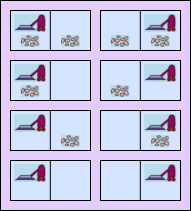
\includegraphics{Pics/ComS472_410.png}}
%\caption{Belief states recheable from initial 8 belief states.}
%\label{Belief states recheable from initial 8 belief states.}
%\end{figure}

\end{document}

















